\begin{appendices}


\titleformat{\chapter}[block]{\bfseries\Large\raggedright}
        {\chaptertitlename{}~\Alph{chapter}.}{1ex}{}
\titleformat{\section}[block]{\bfseries\large\raggedright}
        {\Alph{chapter}.\arabic{section}}{1ex}{}
%\titleformat{\subsection}[block]{\bfseries\normalsize\raggedright}
%        {\Alph{section}.\arabic{subsection}.}{1ex}{}

\titlecontents{chapter}% <section-type>
  [0pt]% <left>
  {\addvspace{.7pc}}% <above-code>
  {\bfseries\appendixname\ \thecontentslabel\quad}% <numbered-entry-format>
  {\bfseries}% <numberless-entry-format>
  {\bfseries\hfill\contentspage}% <filler-page-format>


%\addtocontents{toc}{\protect\renewcommand{\protect\chaptername}{\appendixname}}

\chapter{Когномены, праздники и храмы Фортуны в Риме}

\section{Когномены Фортуны}

Ниже перечислены когномены Фортуны, которые рассматриваются в настоящем исследовании. Когномены приведены в алфавитном порядке в той форме, в которой они фигурировали (или предполагается, что фигурировали) в культовой практике. В скобках приводится греческая форма имени, если таковая встречается в грекоязычных источниках. Указывается, если известно, форма культового сооружения: храм (\textit{aedes} или \graeca{>ier'on}), святилище (\textit{templum}) или алтарь (\textit{ara} или \graeca{bwm'os}). Знаком вопроса отмечены те культовые сооружения, чьё существование известно только по сообщениям Плутарха, отчего является гипотетическим (см. подробнее п.~\ref{PlutarchiCritica}). Через тире указан номер главы в исследовании, где рассматривается история соответствующего культа.

\begin{enumerate}

\item Adiutrix "--- \ref{FortunaTutela}.
\item Averrunica (\graeca{>apotropa'ios}), \graeca{>ier'on} (?) "--- \ref{FortunaeVariaePlutarchi}.
\item Balnearum "--- \ref{FortunaBalnearum}.
\item Barbata "--- \ref{FortunaBarbata}.
\item Bona "--- \ref{FortunaBona}.

\item Bonae Spei (\graeca{e>u'elpis}), \graeca{>ier'on} (?) или \graeca{bwm'os} в Длинном Переулке (Vicus Longus) на Квиринале (?) "--- \ref{FortunaeVariaePlutarchi}.

\item Brevis (\graeca{mikr'a}), \graeca{>ier'on} (?) "--- \ref{FortunaeVariaePlutarchi}.

\item Cancensis "--- \ref{FortunaeFamiliarum}.

\item Crassiana, \textit{ara} "--- \ref{FortunaeFamiliarum}.

\item Equestris, \textit{aedes} "--- \ref{FortunaEquestris}.

\item Flavia "--- \ref{FortunaeFamiliarum}.

\item Fors Fortuna, \textit{aedes}, у I и VI милевых камней Кампанской дороги и в садах Цезаря "--- \ref{FortisFortunae1}, \ref{FortisFortunae2} и \ref{FortisFortunae3}.

\item Fortuna et Mater Matuta in foro Boario, \textit{aedes} "--- \ref{FortunaInForoBoario}.

\item Horreorum "--- \ref{FortunaHorreorum}.

\item Huiusce Diei, \textit{aedes} "--- \ref{FortunaHuiusceDiei}.

\item Iuveniana "--- \ref{FortunaeFamiliarum}.

\item Mala, \textit{ara} на Эсквилине "--- \ref{FortunaMala}.

\item Muliebris, \textit{aedes} или \textit{templum} или \graeca{<ier'on} у IV милевого камня Латинской дороги "--- \ref{FortunaMuliebris}.

\item Obsequens (\graeca{meil'iqia} или \graeca{peij'hnia}), \graeca{>ier'on} (?) "--- \ref{FortunaObsequens}.

\item Primigenia Publica Populi Romani Quiritum in Colle, \textit{aedes} "--- \ref{FortunaPublicaPrimigenia} и \ref{TresFortunae}.

\item Privata (\graeca{>id'ia}), \graeca{>ier'on} (?) "--- \ref{FortunaeVariaePlutarchi}.

\item Publica Citerior in Colle, \textit{aedes} "--- \ref{FortunaPublicaCiteriori} и \ref{TresFortunae}.

\item Rescipiens (\graeca{epistrefom'enh}), \graeca{>ier'on} на Эсквилине (?) "--- \ref{FortunaRescipiens}.

\item Salutaris "--- \ref{FortunaSalutaris}.

\item Torquatiana "--- \ref{FortunaeFamiliarum}.

\item Tres Fortunae, \textit{aedes (tres)} "--- \ref{TresFortunae}.

\item Tulliana, \textit{aedes} "--- \ref{FortunaTulliana}.

\item Tutela "--- \ref{FortunaTutela}.

\item Virgo, \graeca{>ier'on} (?) "--- \ref{FortunaVirgo}.

\item Virilis (\graeca{>'arrenos}), \graeca{>ier'on} (?) "--- \ref{FortunaVirilis}.

\item Viscata (\graeca{>ixeutr'ia}), \graeca{>ier'on} (?) "--- \ref{FortunaViscata}.

\end{enumerate}

\section{Календарные праздники Фортуны в Риме}\label{appendix:festivales}

\begin{itemize}

\item \textbf{1 апреля} (Veneraliae), \textit{Fortuna Virilis} (fasti Praenestini, Ovid. Fast. IV.145--150).

\item \textbf{5 апреля} \textit{Fortuna Publica Citerior in Colle} (fasti Praenestini, Ovid. Fast. IV.375--376).

\item \textbf{25 мая} \textit{Fortuna Primigenia Publica Populi Romani Quirites in Colle Quirinali} (fasti Esquilini, Caeretani, Venusini, Ovid. Fast. V.729--731).

\item \textbf{11 июня} (Matraliae), \textit{Fortuna et Mater Matuta in foro Boario} (Ovid. Fast. VI.568--572).

\item \textbf{24 июня} \textit{Fors Fortuna} (fasti Amiternini, Esquilini, Philocali, Menologia Rustica Colontianum et Valense, Ovid. Fast. VI.771--784).


\end{itemize}

\pagebreak
\section{Схема известных храмов Фортуны}

\begin{figure}[h!]
\center{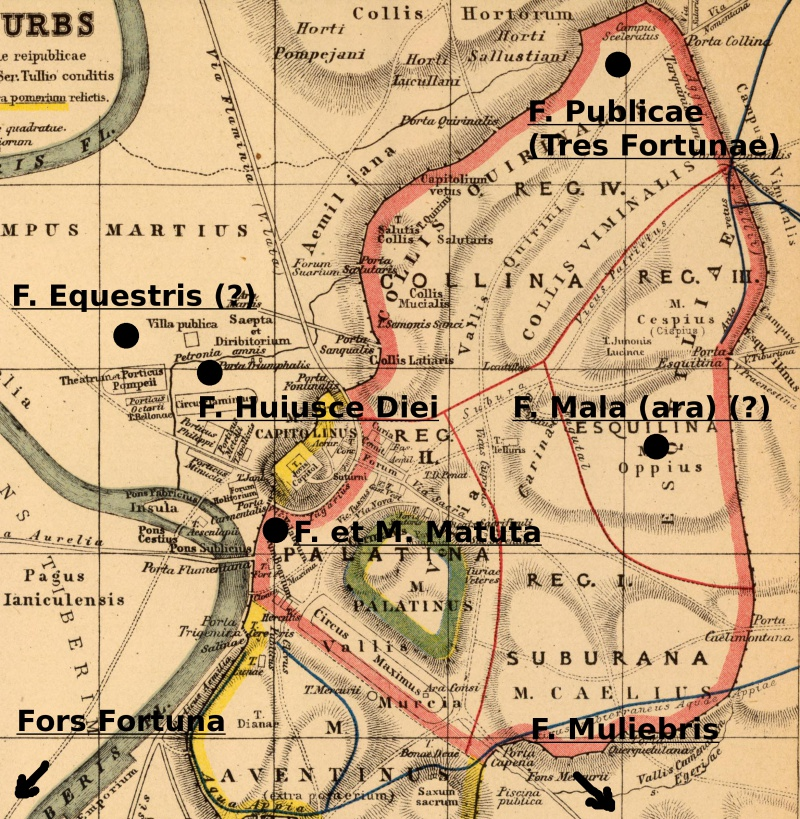
\includegraphics[scale=0.55]{images/roma_map1.jpg}}
\caption{Схема местоположения известных храмов Фортуны в Риме. \footnotesize{Источник оригинальной карты: \cite[Bl. XXII]{Kiepert1894}. }}
\label{pic:Charta}
\end{figure}


\chapter{Археологические свидетельства}

\section{Храм Фортуны на Бычьем форуме}\label{appendix:InForoBoario}

\begin{figure}[ht!]
\center{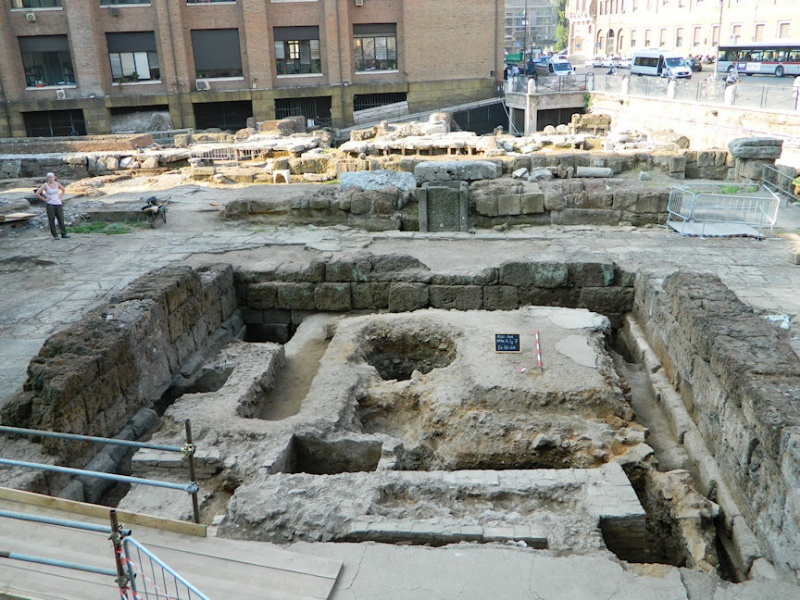
\includegraphics[scale=0.5]{images/figure1m.jpg}}
\caption{Общий вид раскопок в районе Сан-Омобоно. Современное состояние. \footnotesize{Источник: \cite[URL: \href{http://intarch.ac.uk/journal/issue31/1/images/figure1.html}{http://intarch.ac.uk/journal/issue31/1/images/figure1.html}]{Terrenato2012}}
}\label{pic:SOmobono1}
\end{figure}

\begin{figure}[ht!]
\center{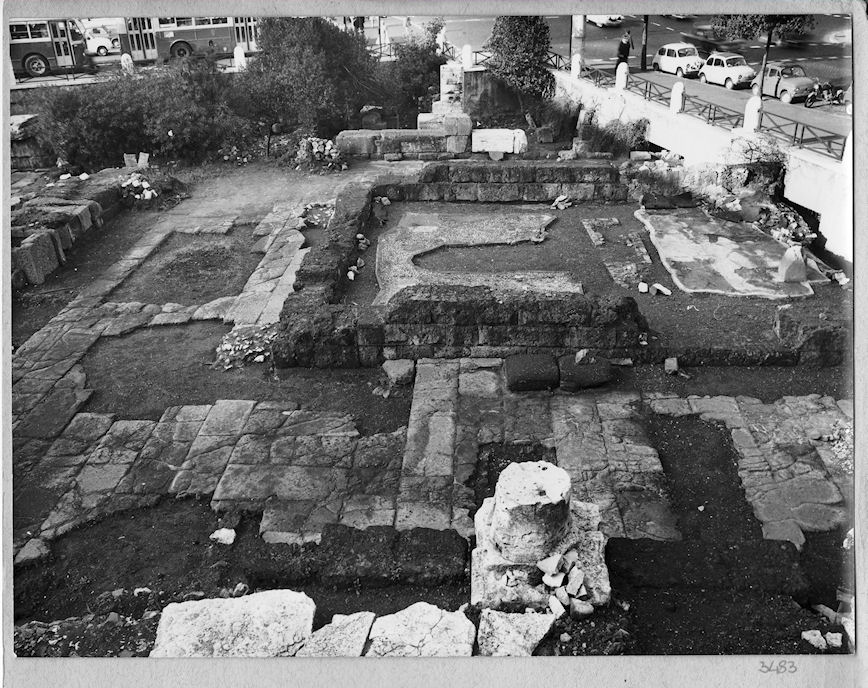
\includegraphics[scale=0.5]{images/figure62m.jpg}}
\caption{Вид на западный храм с запада (AFSRCM, S. Omobono, b. 29, 7, c. 3483).  \footnotesize{Источник: \cite[URL: \href{http://intarch.ac.uk/journal/issue31/1/images/figure62.html}{http://intarch.ac.uk/journal/issue31/1/images/figure62.html}]{Terrenato2012}}. }\label{pic:SOmobono2}
\end{figure}

%\pagebreak

\begin{figure}[ht!]
\center{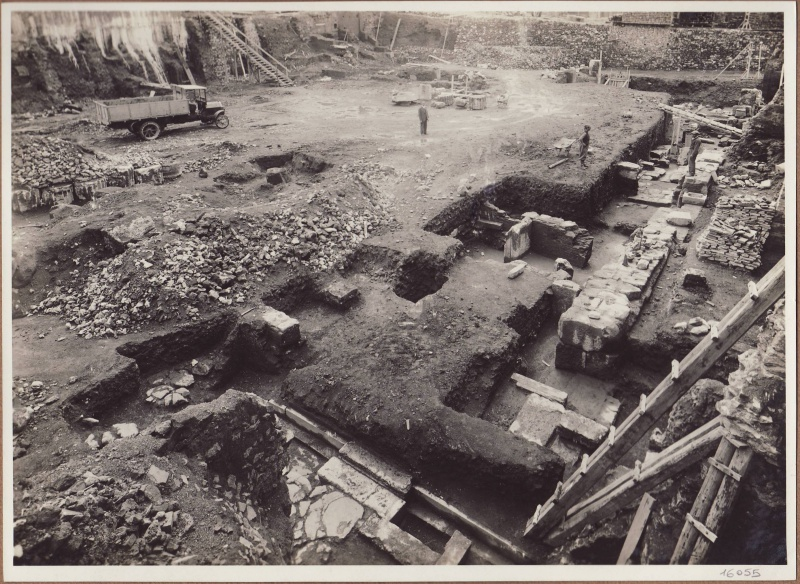
\includegraphics[scale=0.55]{images/figure32.jpg}}
\caption{Раскопки района церкви Сан-Омобоно в 1937 г.  \footnotesize{Источник: \cite[URL: \href{http://intarch.ac.uk/journal/issue31/1/images/figure32.html}{http://intarch.ac.uk/journal/issue31/1/images/figure32.html}]{Terrenato2012}}. }\label{pic:Excavatio1937}
\end{figure}

\begin{figure}[ht!]
\center{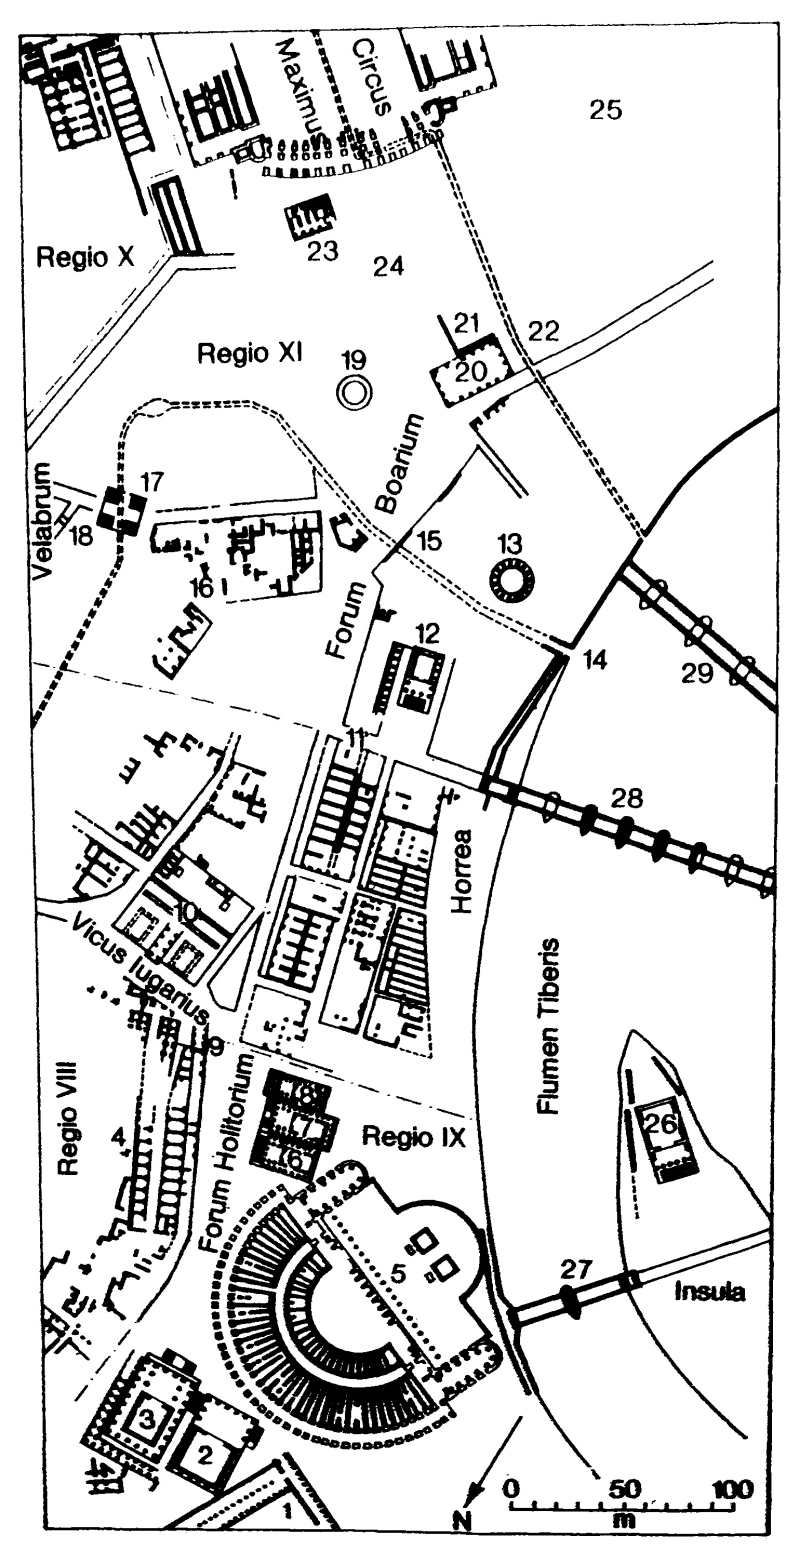
\includegraphics[scale=0.4]{images/fig02.jpg}}
\caption{Схема района Бычьего форума. Двойное святилище Фортуны и Матери Матуты обозначено под №~10. \footnotesize{Источник: \cite[P. 163]{Richardson1992}}. }
\label{pic:ForiBoariSchema}
\end{figure}

\begin{figure}[ht!]
\center{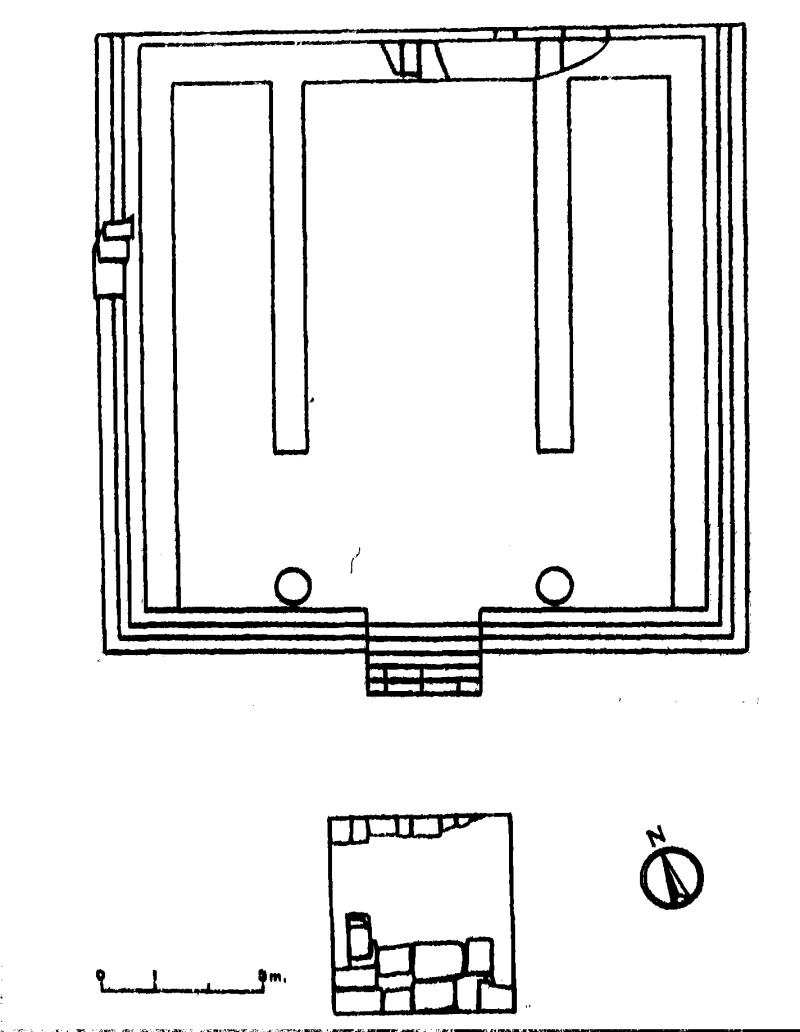
\includegraphics[scale=0.25]{images/fig04.jpg}}
\caption{Схема архаического храма в районе Сан-Омобоно (реконструкция). \footnotesize{Источник: \cite[P. 35]{Richardson1992}}. }\label{pic:ArchaicTemple1}
\end{figure}

\begin{figure}[ht!]
\center{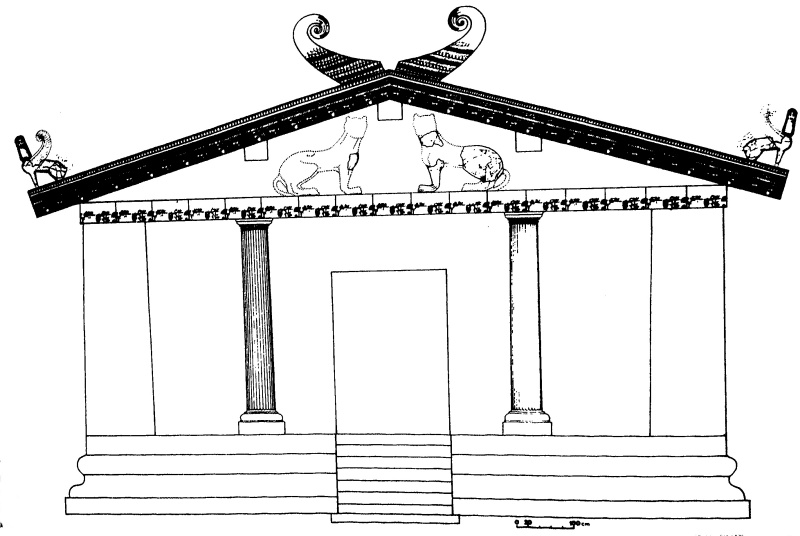
\includegraphics[scale=0.45]{images/fig05.jpg}}
\caption{Внешний вид архаического храма в районе Сан-Омобоно (реконструкция). \footnotesize{Источник: \cite[P. 36]{Richardson1992}}. }\label{pic:ArchaicTemple2}
\end{figure}

\begin{figure}[ht!]
\center{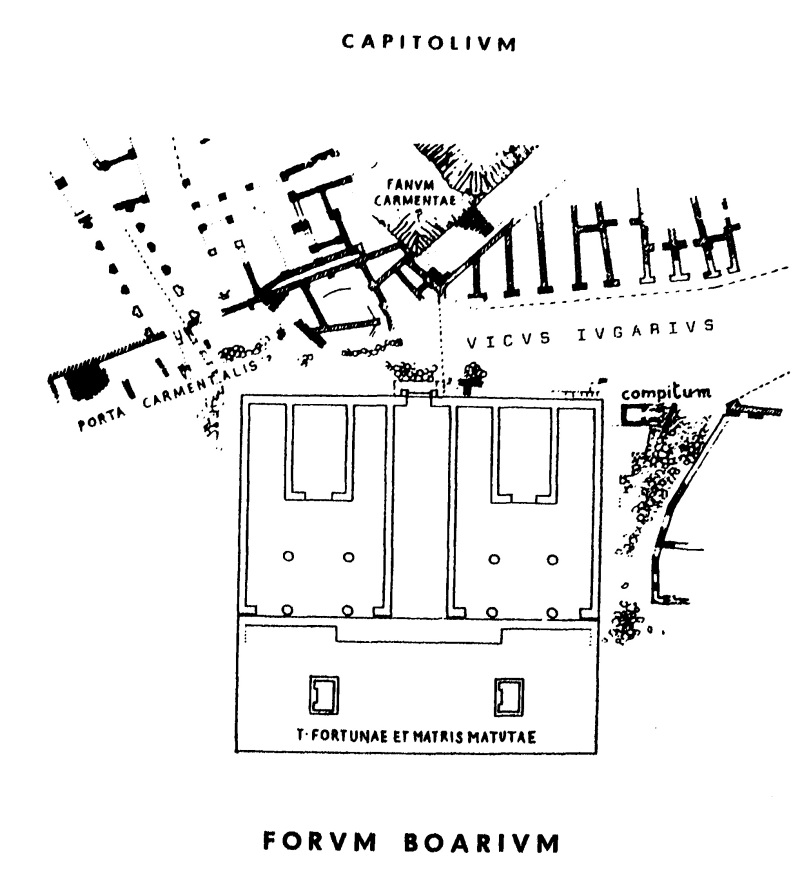
\includegraphics[scale=0.4]{images/fig03.jpg}}
\caption{Схема двойного храма Фортуны и Матери Матуты в районе Сан-Омобоно. Финальная фаза. \footnotesize{Источник: \cite[P. 35]{Richardson1992}}. }\label{pic:TwinTemples}
\end{figure}


\section{Aedes Fortunae Huiusce Diei}\label{appendix:FortunaHD}


\begin{figure}[ht!]
\center{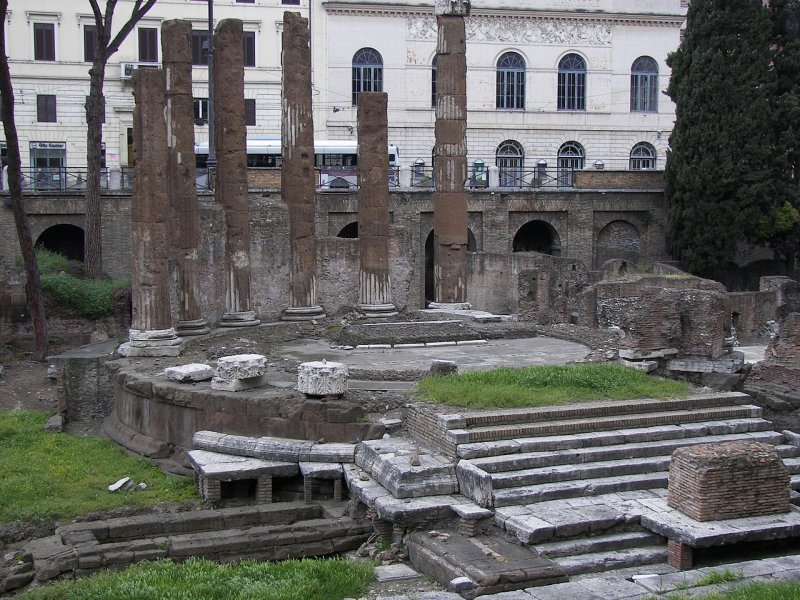
\includegraphics[scale=0.55]{images/forthd.jpg}}
\caption{Aedes Fortunae Huiusce Diei. Современное состояние. \footnotesize{}. }\label{pic:FortunaHD}
\end{figure}

\begin{figure}[ht!]
\center{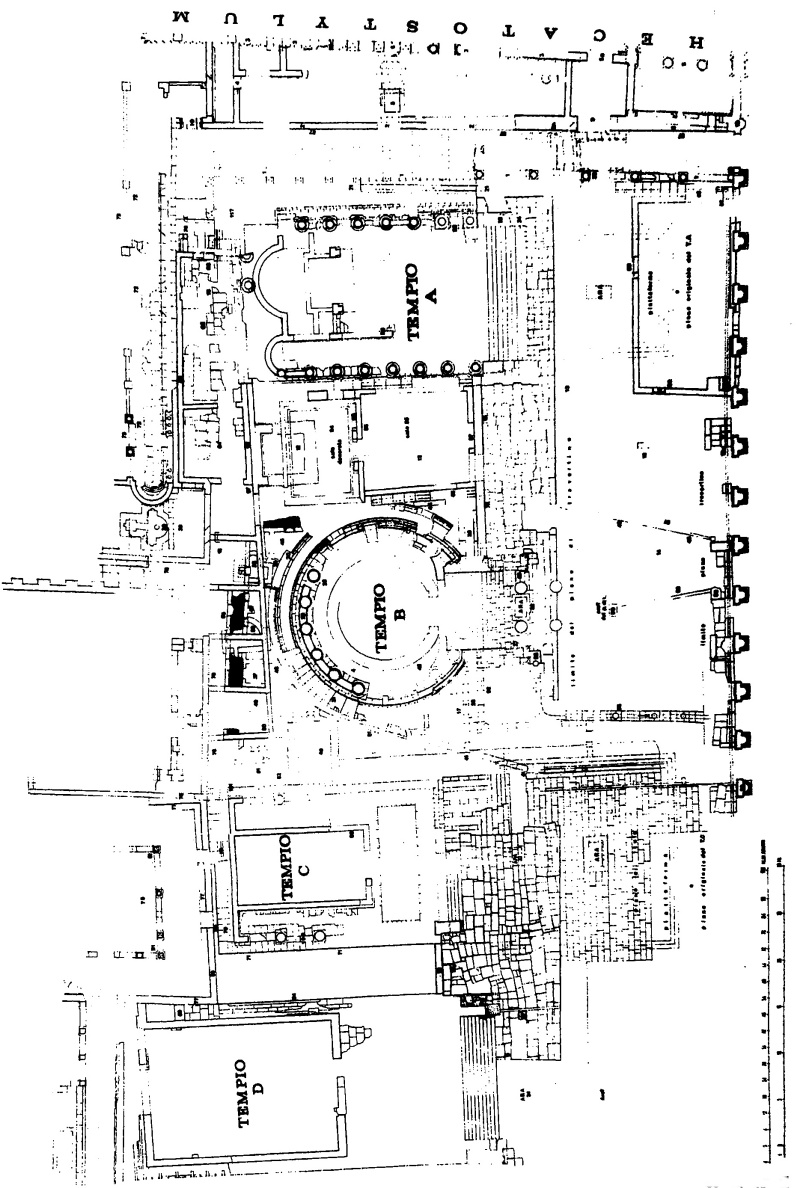
\includegraphics[scale=0.5]{images/forthd1.jpg}}
\caption{Общая схема Area Sacra di Largo Argentina. Храм Fortunae Huiusce Diei обозначен под литерой B. \footnotesize{Источник: \cite[P. 34]{Richardson1992}}. }
\end{figure}

\chapter{Монеты}

\begin{figure}[ht!]
\center{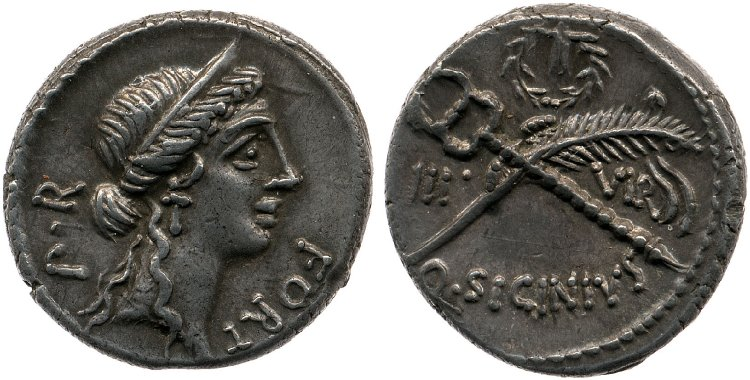
\includegraphics[scale=0.5]{images/RRC_440_1_1.jpg}}
\caption{Денарий с изображением Фортуны Римского Народа. Чеканка Рима, 49 г. до н.э. RRC 440/1. }\label{pic:RRC440}
\end{figure}

\begin{figure}[ht!]
\center{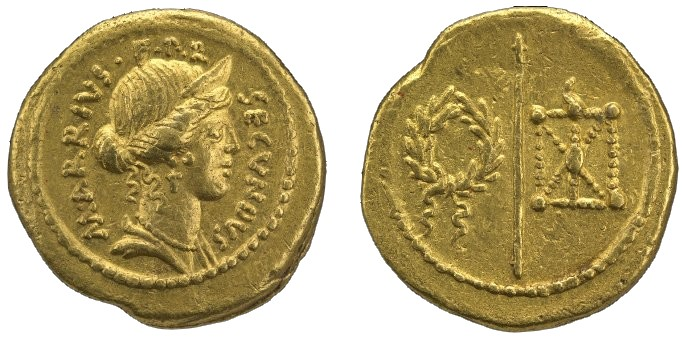
\includegraphics[scale=0.5]{images/RRC_513_1(1).jpg}}
\caption{Ауреус с изображением Фортуны Римского Народа. Чеканка Рима, 41 г. до н.э. RRC 513/1. }\label{pic:RRC513}
\end{figure}

\begin{figure}[ht!]
\center{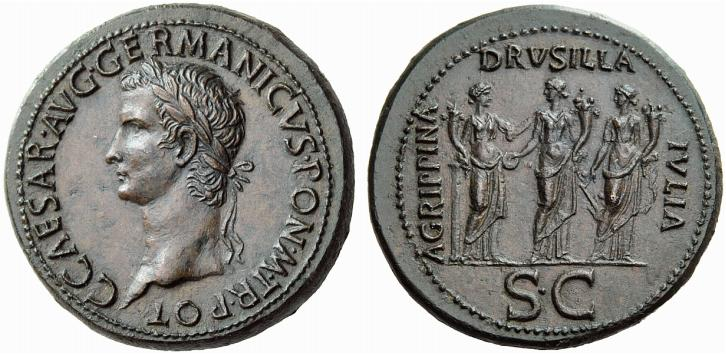
\includegraphics[scale=1.6]{images/ric_I_Caligula_33.jpg}}
\caption{Сестерций Калигулы с изображением трёх его сестёр. Агриппина изображена с атрибутами Секуритас, Друзилла "--- Конкордии, Юлия "--- Фортуны. Чеканка Рима, 37--38 гг. н.э. RIC I, Cal. 33.}\label{pic:CaligulaeSorores}
\end{figure}


\begin{figure}[ht!]
\center{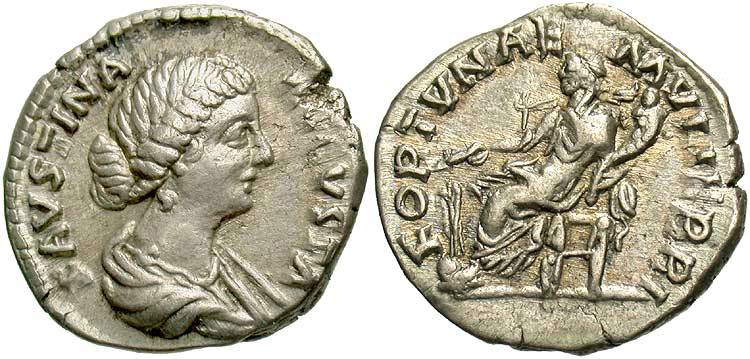
\includegraphics[scale=0.5]{images/RIC_III_Marcus_Aurelius_683.jpg}}
\caption{Денарий Марка Аврелия, посвящённый его жене, Фаустине Младшей, с изображением Женской Фортуны. RIC III, Marc. Aur. 683. }\label{pic:FortunaMuliebris}
\end{figure}

\chapter{Изображения Фортуны}\label{appendix:Pictura}

\begin{figure}[ht!]
\center{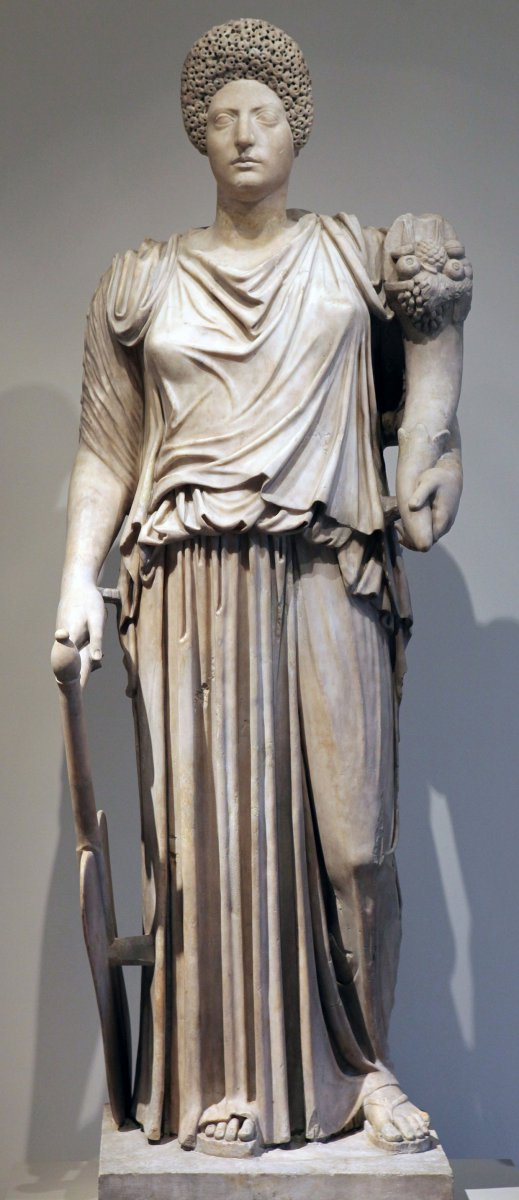
\includegraphics[scale=0.37]{images/sc0030.jpg}}
\caption{Статуя Тихи-Фортуны, мрамор, 2-я пол. I в. н.э. Нью-Йорк, музей Метрополитен. В результате реставрации кон. XVIII в. к статуе была приставлена голова неизвестной женщины (кон. I в. н.э.). \footnotesize{Фото и текст \textit{Роджер Б. Ульрих}. Источник: \href{http://ancientrome.ru/art/artwork/img.htm?id=4038}{http://ancientrome.ru/art/artwork/img.htm?id=4038}}}
\label{pic:FortunaFlav}
\end{figure}


\begin{figure}[ht!]
\center{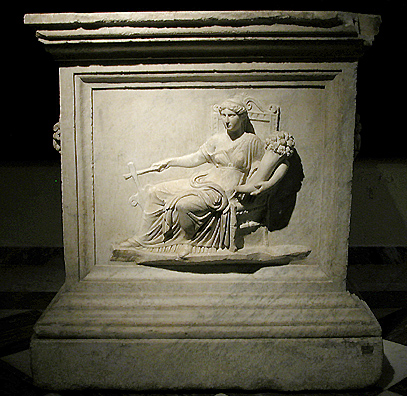
\includegraphics[scale=1.0]{images/ara_fortunae_1.jpg}}
\caption{Алтарь Фортуны, мрамор, датировка неизвестна. Рим, Капитолийский музей. \footnotesize{Фото \textit{Ann Raia}, 2007 г.}}
\label{pic:Ara1}
\end{figure}


\begin{figure}[ht!]
\center{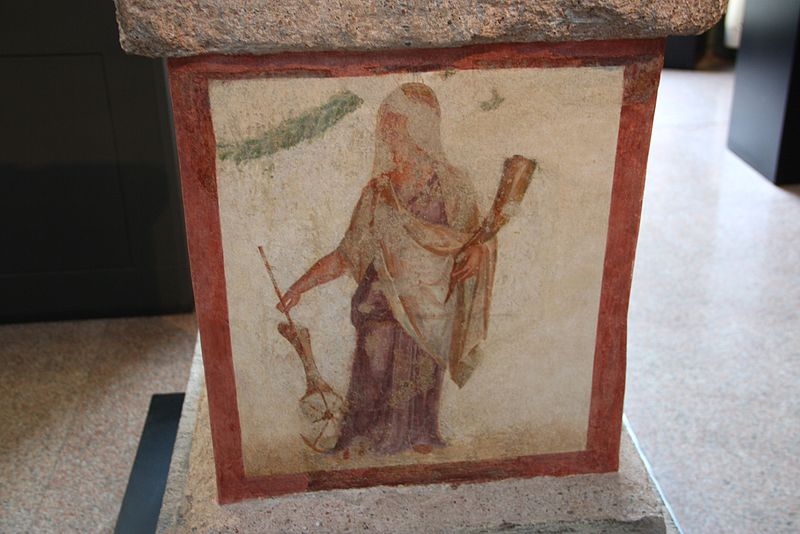
\includegraphics[scale=0.5]{images/ara_fortunae_2.jpg}}
\caption{Алтарь Фортуны, I--II вв. н.э. Миланский музей. \footnotesize{Фото \textit{Ann Raia}, 2007 г.}}
\label{pic:Ara2}
\end{figure}

\begin{figure}[ht!]
\center{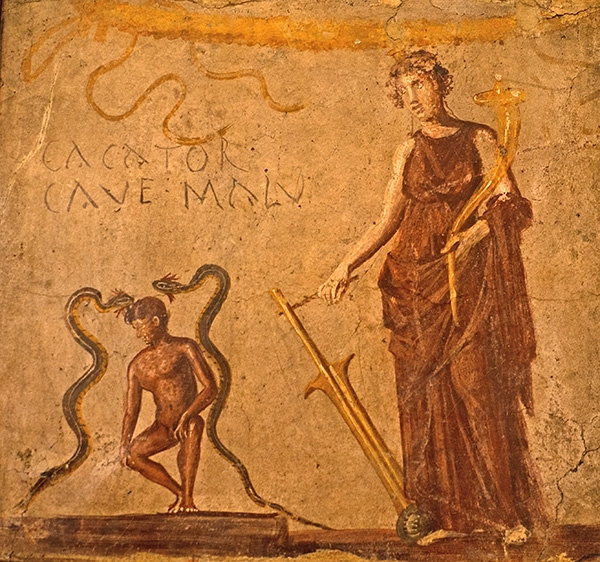
\includegraphics[scale=0.7]{images/cavemalum_fresco.jpg}}
\caption{Фреска с изображением Фортуны, Помпеи, I в. н.э. Неаполитанский музей. \footnotesize{Фото \textit{Barbara McManus}, 2012 г.}}
\label{pic:Cavemalum}
\end{figure}

\begin{figure}[ht!]
\center{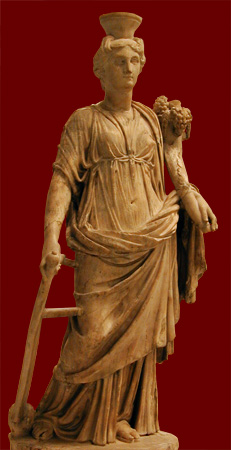
\includegraphics[scale=1.0]{images/fortuna_statue.jpg}}
\caption{Мраморная статуэтка Фортуны, 2-я пол. II в. н.э. Лондон, Британский музей. \footnotesize{Фото \textit{Barbara McManus}, 2001 г.}}
\label{pic:Fortuna2cent}
\end{figure}


\end{appendices}
